
	\paragraph{QuizziPedia::Front-End::AppRouter}
	
	\label{QuizziPedia::Front-End::AppRouter}
	
	\begin{figure}[ht]
		\centering
		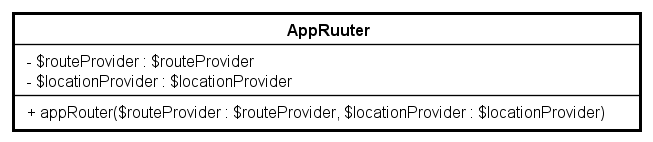
\includegraphics[scale=0.5,keepaspectratio]{UML/Classi/Front-End/QuizziPedia_Front-end_AppRouter.png}
		\caption{QuizziPedia::Front-End::AppRouter}
	\end{figure} \FloatBarrier
	
	\begin{itemize}
		\item \textbf{Descrizione}: classe che gestisce i routes dell’applicazione, utilizza il servizio \texttt{\$routeProvider} per associare ad ogni route un controller e una view;
		\item \textbf{Utilizzo}: viene utilizzata per associare un URL alle varie view dell’applicazione;
		\item \textbf{Attributi}:
		\begin{itemize}
			\item \texttt{\$routeProvider: \$routeProvider}\\ Campo dati contenente un riferimento al servizio di \textit{Angular.js\ped{G}} che si occupa di definire le route dell’applicazione;
			\item \texttt{\$locationProvider: \$locationProvider}\\ Campo dati contenente un riferimento al servizio di \textit{Angular.js\ped{G}} che si occupa di configuare come i paths vengono memorizzati.
		\end{itemize}
		\item \textbf{Metodi}: 
		\begin{itemize}
			\item \texttt{+} \texttt{AppRouter(\$routeProvider: \$routeProvider, \$locationProvider: \$locationProvider)}: metodo che gestisce i routes dell’applicazione. Utilizza il servizio \$routeProvider per associare ad ogni route un controller e una view; e \$locationProvider per configurare come i paths dell'applicazione vengono salvati. Questa funzione viene utilizzata come parametro nel metodo texttt{config} di \textit{Angular.js}. Il metoto \texttt{config} permette di impostare l'esecuzione di una funzione al caricamento del \textit{modulo\ped{G}} principale di \textit{Angular.js\ped{G}};
			\textbf{Metodi}:
			\begin{itemize}
				\item \texttt{\$routeProvider}: campo dati contenente un riferimento al servizio di \textit{Angular.js\ped{G}} che si occupa di definire le route dell’applicazione;
				\item \texttt{\$locationProvider}: campo dati contenente un riferimento al servizio di \textit{Angular.js\ped{G}} che si occupa di configuare come i paths vengono memorizzati.
			\end{itemize}
		\end{itemize}
	\end{itemize}
	
